\chapter{Versioning}
\label{chap:versioning}

Versioning determines creation of releases of a product and its management. The product is what provider offers to consumer. A new version of product is created when a modification is needed. Consumers can use the same product but they can use its different version. The version could have been released because of new requirements or due to improvements of functionality. 

Any of new versions of the product mustn't influence the execution of consumers code. When the product is customized, a change has to be compatible with all consumers. In case the change is incompatible, it is needed to release a new version. Before a consumer switches the new version an agreement between provider and consumer has to be established. The consumer has to do required changes within his functionality deriving from the new agreement.

A change which leads to necessity of modification on consumer side can be a new requirement from one of the consumers, the new version is released and the consumer can immediately switch to use it. Other consumers can follow their schedule and switch to the newest version when it is suitable for them. 

In service oriented architecture the product are services as they are descibed in section \ref{sec:services}. Provider is one who provide services, server. Consumer is one who use services, client.

\section{Version compatibility}
\label{sec:v-compat}
There are two forms of versioning concerning compatibility. \cite{website:service-versioning}
\begin{description}
  \item[Compatible changes] \hfill \\
  Compatible changes are that changes of product which do not harm any consumer. Compatible changes are for example implementation bug fixes or change in number of parameters in interface to support an implementation modification.
  \begin{enumerate}
    \item[Backward compatible] \hfill \\ 
  When a new version of a service is deployed the consumer of an earlier version must be capable to interoperate with the new version without any modification of his application. If a service is backward compatible it is compatible with older version of itself. Backward compatible change can be an addition of a new resource or a new capability to the resource. \hfill \\ 
  Example: \hfill \\ 
  Service has capability \hfill \\ 
  \begin{lstlisting}
  GET   /customers/{customerId}
  \end{lstlisting}
  and we add a new capability to get only the name of a customer with assigned id
  \begin{lstlisting}
  GET   /customers/{customerId}/name
  \end{lstlisting}

  This addition doesn't harm any consumer of the service, because they can continue to use every capability which has been already integrated in their systems. Every capability is still a part of the new version of the service. 
  
  \item[Forward compatible] \hfill \\
  The service version is forward compatible when it is designed in a way it can support future modifications. The newer version of service can be deployed without influence on its usability by consumers. 
  \end{enumerate}
  
  \item[Incompatible changes] \hfill \\
  Incompatible changes are breaking changes which affect consumers of services. An example is removal of an action or change of types or order of parameters of an action.
  \begin{enumerate} 
    \item[Backward incompatible changes]  \hfill \\
    Backward incompatible changes are changes which break the consumers using an earlier version of service. It means that the new version is no longer backward compatible and do not interpret the data of its earlier version.
    \item[Forward incompatible changes] \hfill \\
    These changes break the forward compatibility of the service. It means that a future version won't be compatible with existing one, any modifications of current version don't preserve compatibility.
  \end{enumerate}
\end{description}

\section{Versioning of services}
\label{sec:verioningservices}
Thanks to versioning services can be evolved and customized. When a breaking change of a service occurs the new version can be created so that existing consumers of services are not affected. Release of a new version doesn't harm the previous one, all versions can coexist and be used at the same time. 

\subsection{Versioning on different levels of a service}
As there are three levels of interpretation of a \emph{service} as was already described in section \ref{subsec:levels-of-service}. A change and consequent creating of a new version can occur within each of this levels - business abstraction, service interface and service implementation.

\subsubsection{Versioning of service implementation}
The implementation of a service can be changed. The new version of service is backward compatible or backward incompatible. The backward compatible modification in this level is simple bug fix, the incompatible changes are changes which affect the interface of the service.

The implementation is encapsulated under the interface and it is not visible for outer world. Despite this the implementation cannot be replaced without affecting the whole service. A provider of service has a contract including \gls{sla} with a service consumer. The contract has to be followed because it is valid document on which the consumer relies. 

Every change which has to be done in the implementation of the service needs to be validated against the contract. When the implementation which is going to be replaced is the breaking change from the point of view of the consumer the agreement with the change of contract is needed and consequently the new version has to be released.

Changes of the implementation lead to the versioning of the code. Compatible changes can be done without necessity of new version, but they should be versioned after specific amount of changes (this amount should be specified as a part of versioning strategy) for proper change management. In case of a breaking change, the code has to be versioned.

\subsubsection{Versioning of service interface}
As mentioned service interface is an entry point for consumers to work with the services. Interface can be versioned as well and its change has impact on the consumer application. Compatible changes of the interface are for example addition of an action on the other side non compatible change is removal of an operation. When a new action is added no one is using it and it is optional if somebody would make use of it. When an action is removed, consumers which have used it are broken.

\emph{Service interface versioning} is the interpretation which will be further described and analysed. It brings various approaches with their advantaes and disadvantages. The versioning of services is quite young topic and there are still very vibrant discussions about the best approach.

\subsubsection{Versioning of business service}
Sometimes it is needed to change the business service. It means the business which is abstracted have to be changed. For example because of new requirements due to legislative a business service needs modifications, if this kind of change affects behaviour, semantic or functionality modification of existing service it is easier to create a new service rather than a version. 

\section{Versioning strategy}
\label{sec:version-strategy}
There is a need to specify a set of rules to version services consistently. This rules form the versioning strategy. They are related to release of a new version of services or number of services which should be active at the same time. The rules are the matter of SOA governance. There isn't single correct way to govern the service versioning. Defined strategies should be followed and practiced during whole service lifecycle \cite{soa-governance}:

\begin{description}
  \item[Strict]  \hfill \\
  Any change of a service results in a new version. This strategy does not support backward or forward compatibility.
  \item[Flexible] \hfill \\
  Any incompatible changes result in a new version and the service design supports backward compatibility.
  \item[Loose] \hfill \\
  Any incompatible changes result in a new version and the service design supports backward and forward compatibility.
\end{description}

The strategy needs to be determined during the analysis stage of application lifecycle. It includes more decisions regarding versioning which have to be done before the service implementation such as version identification by digits or version lifecycle.

\subsection{Version identifiers}
\label{subsec:versionid}
Identification of the version is one of the fundamental design patterns. Version is indicated by decimals separated by periods. The version number length and common meaning of the digits should be established as a part of the versioning strategy. Every digit increments releatively to significance of the change. It is usually composed from two to four digits X.Y.Z.R.

Explanation of the digits \cite{soa-governance}:

\begin{enumerate}
  \item[Major changes X] \hfill \\
  Major changes are non-backward compatible changes, after a major change the new document schema is no longer compatible with the old one. These changes break the usage of the service by the consumer. They are imposed to the new version and consumers need to adjust their programs to switch to this version. Breaking changes can be performed by adding or removing an enumeration, removing or renaming a global type or element, changing the optionality of an element from optional to required.
  
    \item[Minor changes Y] \hfill \\
  Minor changes are backward-compatible changes. The changes do not impact consumers, the new version continue to support the consumers working with the old version. Examples can be new optional element to existing type, a change of optionality of a local element from required or optional, adding global type or global element, etc.
  
  \item[Patch version Z] \hfill \\  
  Patch version Z is incremented if only backwards compatible bug fixes are introduced. A bug fix is defined as an internal change that fixes incorrect behavior.
  
  \item[Revisions R] \hfill \\ 
  Revisions are changes without semantic content, for example formatting, comments, etc. They do not affect the functionality of the service and service consumers.
\end{enumerate} 

Using version identifiers to express the compatibility by incrementing major and minor numbers serve to compatibility guarantee. There is another approach to indicate the version of services related to amount of work. The number increment according to effort which have been dedicated to the change. The big effort increments the major number and modest effort the minor number. This two approaches can be combined and in most cases they are, preserving mainly the compatibility guarantee and less often communicating the effort made. \cite{soa-governance}


\subsection{Service version life-cycle}
Service life-cycle defines the time period in which a version should be maintained. When the time is short, customers have not enough time for their upgrades required in order to switch on new verion. On the other hand when the period is too long, too many versions of service have to be maintained. The suitable time span is a result of consideration of individual organization with respect to their capability to deal with changes.

Product version should be always compatible with consumers usage. When a new version of the service method is released, it is needed to have the old one present in the implementation if any of the consumers operate with it. When the service method is going to be replaced by new one, it has to be held so that do not impact any consumer. It can be signed as deprecated, which do not influence its usage from the point of view of the consumer, but it means that provider waits that all consumers switch to the new implementation. When the deprecated method stops to be used, it can be safely removed. 

This lifecycle is possible only when the service method versioning approach is implemented, in case of whole-service versioning, when the service is given into state deprecated, it is equivalent to its remove, it is needed the new agreement between the provider and consumer so that consumer have to implement changes to use the new service. %or just keep using the older version. 
The whole-service versioning provides less flexibility.


\section{Versioning approaches}
\label{sec:versioning-approaches}

The service interface can be versioned in more ways. One of the approaches can be deployment of new version to new environment. This approach is widely used for code versioning not only for services. This is how the service implementation is versioned. Regarding service interface it is possible to create new version and deploy it on the same environment as the older one. This is specific approach for sevice interface versioning. Then there is a question how consumer can access the requested version of the service. The possibilities of access them is analysed in chapter \ref{chap:versionaccess}.


\subsection{New version - new environment approach}

The versioning is based on deployment of new version of \gls{api} on a new environment. The deployment process is identical to software deployment. Service changes are deployed on a new environment incrementing the API version number.

\subsubsection{Deploying of changes}
When in an API with version \emph{v1} a change is done the implementation version number is incrementing in minor digit. From the definition in section \ref{subsec:versionid} is obvious that this is backward compatible change. The implemantation than gains for expamle identifier \emph{1.1} The services do not change their interface and their consumers are not harmed. 
When there were a breaking change in services or there is specified number of changes or amount of work done the whole API is released on a new environment. The API version increase in major identifier to \emph{v2} because non-backward changes were done. Consumers of services needs to do required chages to use newer version of services. Than they call services using new environment. 
The API is usually signed by an major identifier so that on an environment there can be deployed \emph{API v1} or\emph{API v2} and so on.
The implementation of API is versioned using minor, path and revision identifiers. The implementation which is deployed on the server than can have a version for example \emph{1.0.0.0} or \emph{1.3.1.2}. The number insreases depending on what kind of changes was done on the implementation.

\subsubsection{Deployment principles}
The deployment goal is to deliver a high quality product to the consumer. How to reach it is in responsibility of depoyment management and their strategy. The ideal state is when the deployment is simple and fast. To obtain this the changes deployed should be small and should happen often and the new version should be well tested before depoyment to production environment.

\subsubsection{Environments}
To get the quality API it is quite necessary to have more than one environment running the same version of API. Every evnironment has it role and how many of them the producer use is one of the management decisions. At least there are two of them - development and production. Development environment is one with te latest version of API and production environment contains a stable version of API used by consumers.
Better solution is to have more than just this two environmnets. There should be at least one environment dedicated to testing and one environmnet can hold a stable version version of API from which runs the releases to production environment. The last one is generally named as staging environment. It simulates the production environment so that provide to producer test environment of real running of the API discovering system failures before the main release to the production.

One environmnet hold just one version of API. If another version is needed to be available it has to be deployed on another server. Then customers are using different servers, as shown on the image \ref{fig:consumer-server}

\begin{figure}[htp] \centering{
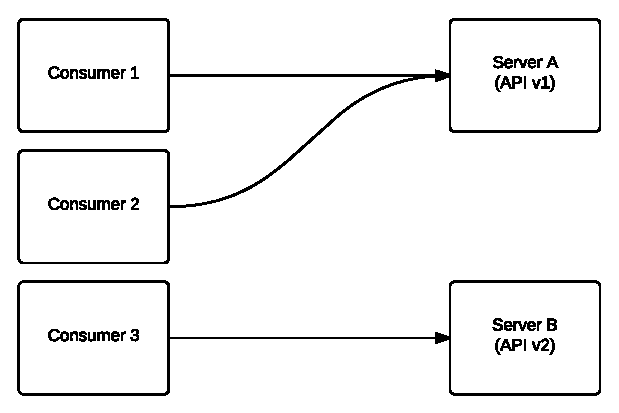
\includegraphics[width=10cm]{img/consumer-server.pdf}}
\caption{}
\label{fig:consumer-server}
\end{figure} 

\subsubsection{Deployment strategy}
One of the approaches how to release a new version of API is cutover, the other one is parallel development. The cutover requires downtime period planing determining when a cutover occurs. 

The parallel deploymnet allow to have more vesions on which the development, testing and consuming are proceeding. This approach offers more reliability, because of running backup system but requires more effort from provider and consumers. When a new version of system is going to be released it is deployed on environmnet but keeping the old system running on its enivoronment and continue with development, support and consuming of the old one. 

Having cutover approach when the actual version of API on the development environment is going to be emitted to the production the developed code version number increases and directly start the development on a new version. The cut version is, after being stable, released to the production. Consumers connect to production environment to use services. The process of deployment can be seen at the Figure \ref{fig:soa-architecture}


\subsubsection{Deployment methods}
There are more possibilities how to deploy the API on the environment. The examples of some methods are file copy method, source code control method and installer method. 

\begin{description}
  \item{File copy method} \hfill \\
  The API image is copied to new environment manually. This method is network based and provide diminuition of distribution time and asistance in updates. On the other hand the there can be problems with accessing the files on network and other with determining the reason of possible system fails. 
  \item{Source code control method} \hfill \\
  There is a possibility to use \gls{SCCS} (SCCS) to assist the distribution of the system. On SCCS server id deployed the master version of the API, developers work with its local version and after making some changes they push them to the server. Having the most recent version depends just on simple update from SCCS server to get the last revision (what is revision was explained in section \ref{subsec:versionid}). 
  \item{Installer method} \hfill \\
  Both of the metods above requires the more of the user effort. This method is more automate. It allows installer techology integration by creating installer package which is distributed and easy to use. Aside this benefits this methods struggles with the minor chages distribution because the new installation package has to be rebuilt.
\end{description}


\begin{figure}[htp] \centering{
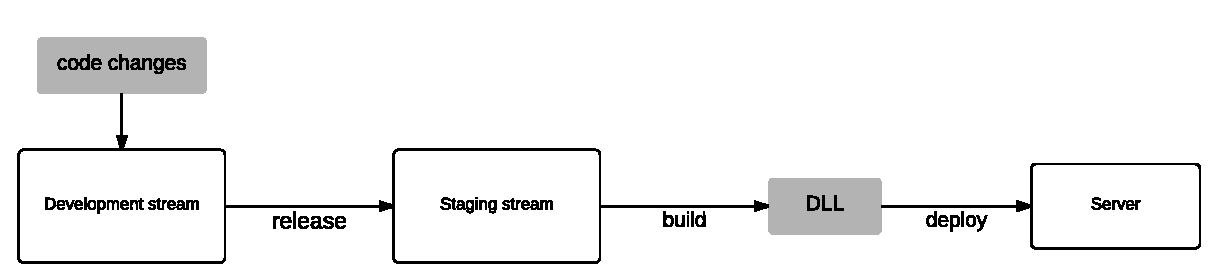
\includegraphics[width=13cm]{img/service-implementation.pdf}}
\caption{Process of deployment of implementation changes}
\label{fig:service-implementation}
\end{figure} 

\subsubsection{Access to versions}
Consumers are always calling just one version of the API, the one which is deployed on the environment against with they are calling the services. They can swith she version of API only if they have the old version on one of the production streams, without changing the URL, just changing the environment. 

\subsubsection{Advatages and disadvatages}
Advantage of this approach is the access to the version. Consumers request sent to the server doesn't change except the integration changes concerning the new version service interface. He has accessible one expected version of API.
From versioning of services part of view the main disadvatage of this approach is the incapability of easily repair inconveniences within the previus version of API. When the API is in versions up to \emph{v3} in development environment and in versions up to \emph{v2} in production environment. When an error is found in production in \emph{v1} this bug is probably supposed to be present also in later versions \emph{v2} and \emph{v3}. Then the bug has to be fixed in all three versions and redeploy them on servers which is not trivial operation.

\bigskip


\subsection{Service interface versioning approach}

Services offers another approach to versioning besides the explained above. There can be runing more than one version of the service API on the same time. This approach can be implemented using various principles. \emph{Service interface versioning} is the interpretation which will be further described and analysed. It brings different principles how to be accessed with their advantages and disadvantages which wil be explained in chapter \ref{chap:versionaccess}.

This versioning approach allows to make changes to the API and release its new version without waiting for consumers to integrate the changes. All versions can run concurrently and be accessed by clients. When there are two coexistent versions of API, \emph{v1} and \emph{v2} consumer can have access to both of them. According to what he sent in the request he is directed to the correct version. Every of this version can be on the same environment or can be separated but this concept the consumer doesn't see.

%Each version has its own implementation and is distinguishably addressed.

%Versioning management of services requires the proper definition of following concepts \cite{website:versioning-in-soa}:
%what will be versioned and how, the life-cycle of the versions and the access to the version.
%\begin{enumerate}
 % \item Units of versioning
 % \item Service changes, constituting a new version
 % \item Service version life-cycle considerations
 % \item Version deployment/access approaches
%\end{enumerate}

\subsubsection{Units of versioning}
\label{sec:units}

The service layer of an application developed by provider is an \emph{API} containing \emph{services}. Services contain \emph{methods (actions)} which ensure operations over the services. The relationship between this entities is shown on Figure \ref{fig:service-layer-design}

\begin{figure}[htp] \centering{
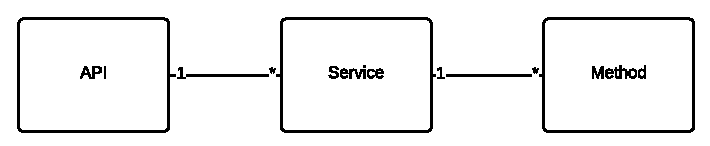
\includegraphics[width=11cm]{img/service-layer-design.pdf}}
\caption{Design of service layer}
\label{fig:service-layer-design}
\end{figure} 

There are three possibilities of what can be versioned in service interface - versioning of \gls{api}, services contained in project or service methods. The relationship between this is shown in Figure \ref{fig:service-layer-design}. The granularity of versioning can be defined by the change which is the reason of creating of a new version. If the change happens just in changes it is possible to version just the method on the other hand when a set of services are changed the whole API should be versioned. These are not rules but the decision what to version should be originated in versioning strategy. The three options can be interchanged should be done carefully to don't complicate services architecture.

Version identified by number which is typically just major digit for each of the version unit. For example the API can be in version \emph{v2} and can contain a service with version \emph{v1} and \emph{v2}, this service versions can have a method of versions \emph{v1} and \emph{v2}.

/obrazok

\begin{description}
\item{Versioning of API} \\
The API containing all services can be versioned. Having the version \emph{v1} API is incremented to version \emph{v2}. This new version can be deployed on the same environment which was running the API v1. Consumers can access them both. Change of API influneces every consumer.
\item{Versioning of service} \\
  The whole service is versioned with all its methods. Versioned servise with version \emph{v1} is changed to \emph{v2}. It can be still part of the API \emph{v1}, just the service version is incremented. When the new version on the service is deployed on environment both service versions can be accessed. The changes influences just consumers which were using the service.
\item{Versioning of service method} \\
  In most cases the change arises just in a method or some methods of a service. It is not necessary to version the whole service, but there is an option to version just these operations. \\
  The benefits of this approach are less code which is deployed because just a changed methods are redeployed in a new version. Services remain unchanged, their name and classification, when there is a method added. The changes concern just a consumers which use the method, instead of consumers of the service containing changed method. \\
  When the versioning of method is used it is needed to deploy each method with its own endpoint address, the advantage is that the \gls{sla} is provided for the method so that it is not changed the SLA of the same service.\\
  Moreover the addressing schema becomes more complex, the consumer has to specify not just the service but also the method and version of method which wants to use.
  In spite of the more elaborate routing this possibility of versioning offers more flexibility. It adapts the services versioning to versioning practices of commonly used programming languages. \\
Other benefit of this versioning unit additing and removing of methods in a service. New method new can be added without any impact on existing consumer. Regarding the removal of a method, there is a deprecation concept. A method which has been for exapmle replaced by new version can be signed as deprecated. A deprecated method takes part until there are still consumers which are using it. When all consumers stop to use it the method can be removed.\\
  Version of changed method \emph{v1} increase in \emph{v2}, this method can be for example part of the service of \emph{v2} and API \emph{v1}.
\end{description}

\subsubsection{Logic of service versioning}
There is a version od the API which is already used in production when there is a breaking change the implemention of new version of API is integrated with the old one. Both version can be deployed into production, it is not mandatory they are on the same environmnet. Consumer can continue to use the old version and after integrating the changes whenever he can switch the version. It is needed to be clear in advance where the version will be places and how will be accessed.
Depending on the principle of accessing the version there can be said explicitly in endpoint address (URL) which version of API, service or method is called. The request is directly roated to requested version. The other approach to have the same endpoint address for each version of the versioned unit and the roating than pass through an intermedia which resolves the correct version, decision is based on one of the parameters send in request. Option of accessing the version will be described in Chapter \ref{chap:versionaccess}.

\subsubsection{Environments}
There are multiple ordered environment begining with the development and ending with production, same as in the implemetnation versioning (new version has always new environmnet) described above. The number and importance od environment is a question of development strategy. For example there can be developmnent environment, some test environments, staging and production environment. 

\subsubsection{Advatages and disadvatages}
The advantage is the version access at any time after deployment in production, the proces in not dependent on consumers integration. The other very significant advatnage is the fixing of failures, ???
On customer site the disadvantage is the forcing to add the version identification in the requests, he has to change it everytime he change the version of API or its subunits. For provider it is needed to implement a logic of acceess different versions.
/TODO



%\subsection{Version definition}
%It is necessary to analyze the services/methods from the point of view of changes, their impact on the consumer. Analysis of possible changes deals with influence of change on the consumers execution and consequently defines the changes which will break it. When the change of the service or method is breaking it leads to the creation of new version.

%The components of the service are interface and message, both of them could be changed and cause the release of new version.

%\subsubsection{Interface changes}
%A change of interface has significant impact on the consumer, it requires many modification of customers implementation or even completely new service. The deprecation of a method is equivalent to its removal and should occur rarely.
%When following semantic messages model, the interface is never changed. Advantage of this approach has source in the fact that all changes can be done just within the methods of service. 
%When the methods are units of versioning they are deployed individually and new methods can be added without any impact on existing consumer. When the method is going to be removed, it is first deprecated, so that is still kept around the service and could be used until all consumers stop to use it. The changes are contained in messages and are not shown within the interface.
%Than as seen it is better to design the versioning definition in order to not include the interface changes.



%\subsubsection{Message changes}
%When using the semantic message model the changes of service interface do not change the interface itself but are contained in message. The message is created by a schema which describes its content. Changes in schema can provide different cases of compatibility with actual implementation and can be divided in three categories:

%\subsection{Version access}
%It is needed to define how different consumers of services are accessing its version of the service. There are several approaches everyone has its pros and cons. The access possibilities are described in separate chapter \ref{chap:versionaccess}.

%\section{Versioning service implementation}
%Besides versioning the service interface, it is possible to consider an implementation. The underlying implementation can changed without affecting the interface itself. 
